\section{Oszilloskop}\label{sec:2}
\subsection{AC-DC Kopplung}\label{sec:2-1}

\begin{highlightblock}[Darstellung eines Rechtecksignals mit AC-DC Kopplung]
	Hier wird die AC- und DC-Kopplung des Oszilloskops verglichen, indem ein Rechtecksignal 
	auf zwei Kanäle mit den unterschiedlichen Kopplungsarten aufgeschalten wird.
	\begin{enumerate}[label=\textbf{\alph*:}, ref=\alph*, noitemsep]
		\item\label{itm:2-P1-1} Kanal 1 auf DC- und Kanal 2 auf AC-Kopplung einstellen.
		\item\label{itm:2-P1-2} Rechtecksignal mit $\SI{50}{\hertz}$ und $\SI{5}{\volt}_{PP}$ Amplitude ohne DC-offset aufschalten.
		\item\label{itm:2-P1-3} Kurvenformen vergleichen. Signale im Zeit- und Frequenzbereich analysieren.
	\end{enumerate}
	
\end{highlightblock}

\subsubsection{Verwendetes Material}

\begin{table}[h]
	\centering
	\caption{Verwendetes Material}
	\begin{tabularx}{\textwidth}{XXX}
		\textbf{Messgerät} & \textbf{Verwendung} & \textbf{Anmerkungen}\\ \midrule
		TDS2014C & Oszilloskop & $Z_E = \SI{1}{\mega\ohm}||\SI{20}{\pico\farad}$ \\
		Agilent 33250A & Funktionsgenerator &  \\
	\end{tabularx}	
\end{table}

\subsubsection{Versuchsaufbau}

\marginref{\ref{itm:2-P1-1},~\ref{itm:2-P1-2}}

Der Ausgang des Funktionsgenerators wird mit einem T-Glied Aufgeteilt und über
Koaxialkabeln mit beiden Kanälen des Oszilloskops verbunden.

\begin{figure}[h]
	\centering
	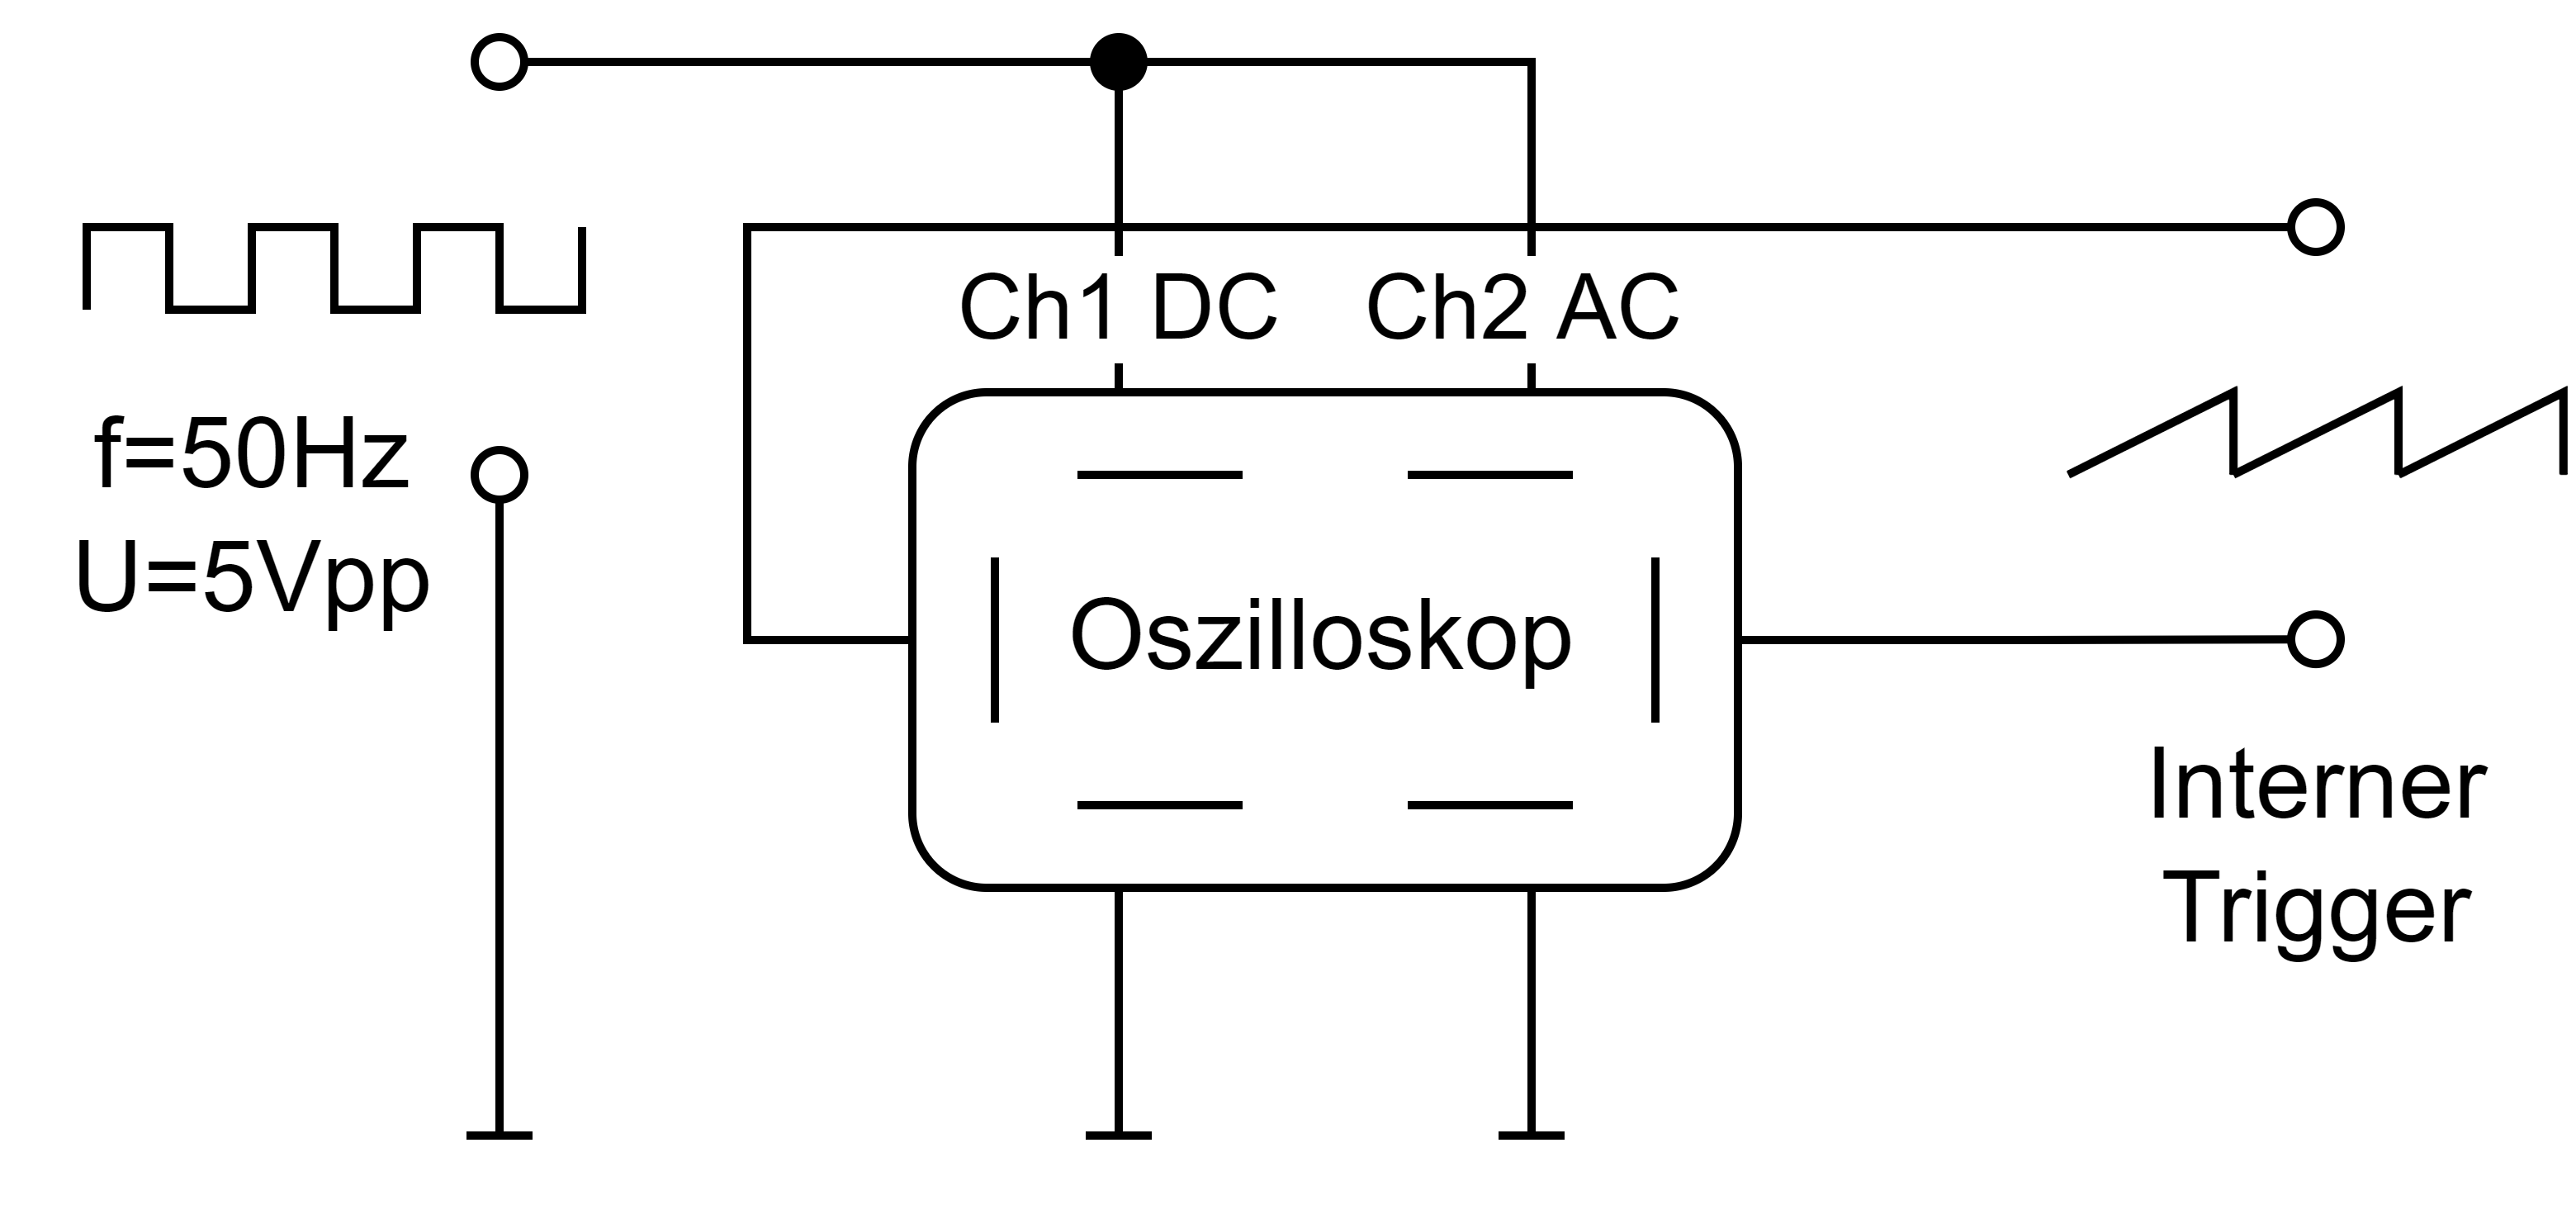
\includegraphics[width=7cm]{images/21_Aufbau.png}
	\caption{Schaltplan des Versuchsaufbaus}\label{fig:21-aufbau}
\end{figure}

Die Geräte werden folgdendermaßen konfiguriert:

\begin{minipage}[t]{.48\textwidth}
Einstellungen des Oszilloskops:

\begin{itemize}[noitemsep]
	\item Kanal 1 (DC): $\SI{2}{\volt}/\text{Div}$, $\SI{2.50}{\ms}/\text{Div}$
	\item Kanal 2 (AC): $\SI{2}{\volt}/\text{Div}$, $\SI{2.50}{\ms}/\text{Div}$
	\item Trigger: Kanal 1, falling edge
\end{itemize}
\end{minipage}\hfill
\begin{minipage}[t]{.48\textwidth}
Einstellungen des Funktionsgenerators:

\begin{itemize}[noitemsep]
	\item Frequenz: $\SI{50}{\hertz}$
	\item Amplitude: $\SI{5}{\volt}_{PP}$
	\item Wellenform: Rechteck
\end{itemize}
\end{minipage}

\newpage
Am Bildschirm des Oszilloskops sind nun die beiden Rechtecksignale zu sehen. 

\begin{figure}[h]
	\centering
	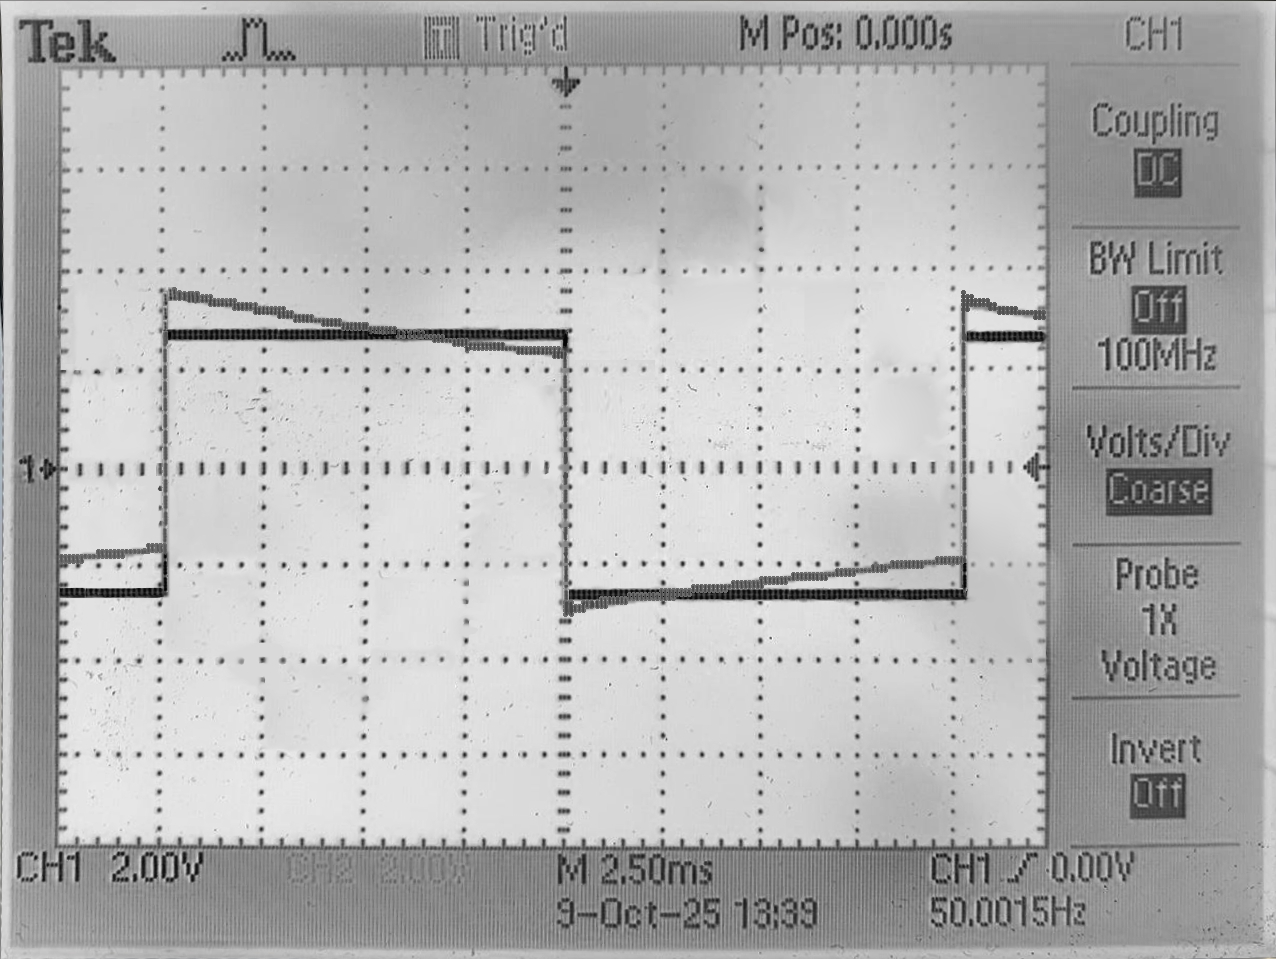
\includegraphics[width=5.5cm]{images/21_AC-DC-oszillogramm.jpg}
	\caption{Oszillogramm des Rechtecksignals beider Kanäle}
\end{figure}

\subsubsection{Erkenntnisse}

\marginref{\ref{itm:2-P1-3}}
Es ist zu erkennen, dass der Kanal mit DC Kopplung das ursprüngliche
Rechtecksignal übernimmt, während der Kanal mit AC Kopplung das Signal verformt.

\textbf{Im Zeitbereich} ist diese Verformung charakteristisch für die Entladekurve eines Kondensators,
welcher sich in Serie zur Messspitze befindet, um Gleichspannungsanteile zu blockieren.

\begin{wrapfigure}[7]{r}{7cm}
	\centering
	\vspace{-25pt}
	\begin{circuitikz}[scale=0.8, transform shape]
		\draw (0,0) node[anchor=east]{$U_\mathrm{E}$} to[C, l=$C_\mathrm{AC}$, o-*] ++(2,0) coordinate (k1)
			to[R=$R_\mathrm{E}$] ++(0,-2) node[rground] {};
		\draw (k1) -- ++(2,0) to[C=$C_\mathrm{E}$, color=lightgray] ++(0,-2) node[rground] {};
		\draw (k1) ++(2,0) to[short, *-o] ++(2,0) node[anchor=west]{$U_\mathrm{A}$}; 
	\end{circuitikz}
	\caption{Eingangsstufe eines AC-gekoppelten Kanals}
\end{wrapfigure}

Der Kondensator $C_\mathrm{AC}$ bildet zusammen mit der Eingangsimpedanz
$R_\mathrm{E}||C_\mathrm{E}$ des Oszilloskops einen Hochpass erster Ordnung. Die
Eingangsstufe des AC-gekoppelten Kanals kann somit durch folgende Schaltung
beschrieben werden. Die geringe Kapazität $C_\mathrm{E}$ des Oszilloskopeingangs
kann in diesem Frequenzbereich vernachlässigt werden.

\textbf{Im Frequenzbereich} belegt ein Periodisches Rechtecksignal alle ungeraden
Harmonischen seiner Grundfrequenz. Die Amplituden der Harmonischen nehmen mit
steigender Frequenz ab. Durch das gegenüberstellen mit der Übertragungsfunktion
des Hochpasses wird ersichtlich, dass die niederfrequenten Anteile des
Rechtecksignals gedämpft werden. Diese Dämpfung macht sich im Zeitbereich als
Verformung des Rechtecksignals bemerkbar.

\begin{figure}[h]
	\begin{minipage}[t]{.48\textwidth}
		\centering
		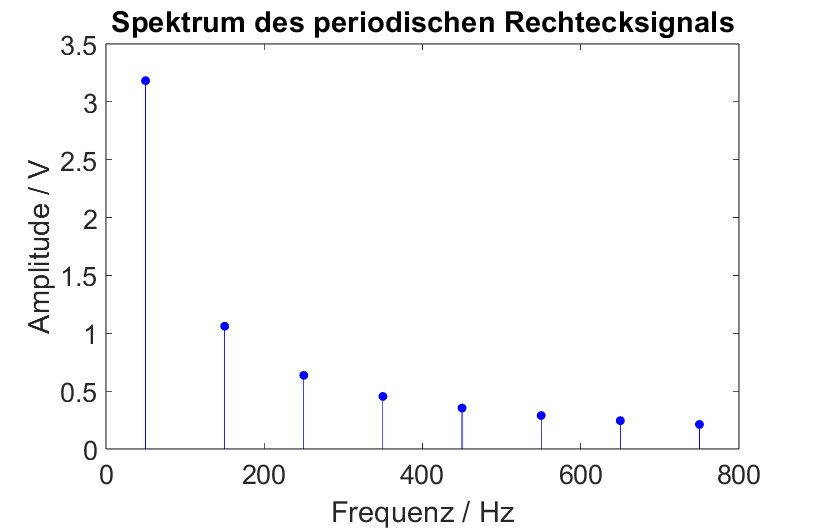
\includegraphics[height=4cm]{images/Spektrum-Squarewave.jpg}
		\caption{Spektrum eines Rechtecksignals}
	\end{minipage}\hfill
	\begin{minipage}[t]{.48\textwidth}
		\centering
		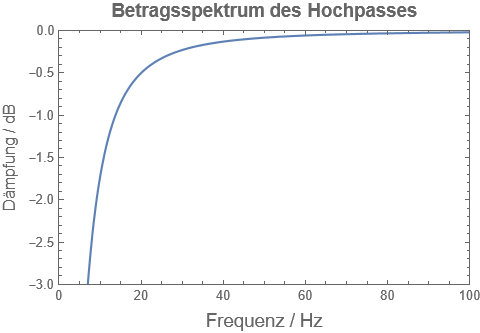
\includegraphics[height=4cm]{images/HochpassAbs.png}
		\caption{Betrag der Übertragungsfunktion des Hochpasses}
	\end{minipage}
\end{figure}